\section{Tekstuel repræsentation af ruter}
\label{sec:tekstuelRepraesentation}

\subsection{Måleenheder}
\label{sec:maaleenheder}

For at vise længden af et vejstykke på en komprimeret og brugervenlig måde, valgte vi at angive længden i forskellige enheder afhængigt af vejstykkets længde. Udgangspunktet var at vise længden i meter, uanset længde, men det viste sig ikke at være optimalt, da det både fyldte meget og var unødigt præcist. Derfor vedtog vi følgende:

\begin{itemize}
	\item Længde vises i meter, hvis længden er mindre end 1000 meter. $L < 1000$.
	\item Længde vises i kilometer med to decimaler, hvis længden er mere end 1000 meter. $L \geq 1000$.
\end{itemize}

\subsection{Retning af vejskifte}
\label{sec:retning}

Vores første idé var at beregne vinklen mellem de to veje, der udgør det enkelte vejskifte, og på den måde afgøre om der er tale om et sving, og i så fald hvilken retning der drejes i. Vi var ikke særlig glade for denne løsning til at starte med, da vi fandt det problematisk, at vi selv skulle definere de forskellige typer sving frem for at aflæse det fra vores data. Denne skepsis forsvandt, efter at vi blev enige om, at vi ikke kunne finde noget data om typen af vejskifte. Valget faldt altså på denne metode, eftersom vi ikke havde noget værdigt alternativ.

Vi besluttede os for følgende definitioner for de forskellige typer vejskifte:

\begin{itemize}
	\item Vinklen mellem to vejstykker bliver beregnet således, at rotation med uret angives med positivt fortegn, og rotation mod uret angives med negativt fortegn.
	\item Hvis vinklen er mindre end 45$^{\circ}$ stor, uanset fortegn, er der ikke tale om et sving. $|A| < PI / 4$.
	\item Hvis vinklen er større end 45$^{\circ}$ og er positiv er der tale om et højre sving. $A \geq PI / 4$.
	\item Hvis vinklen er mindre end 45$^{\circ}$ og er negativ er der tale om et venstre sving. $A \leq -PI / 4$.
\end{itemize}

\begin{figure}[h]
	\centering
	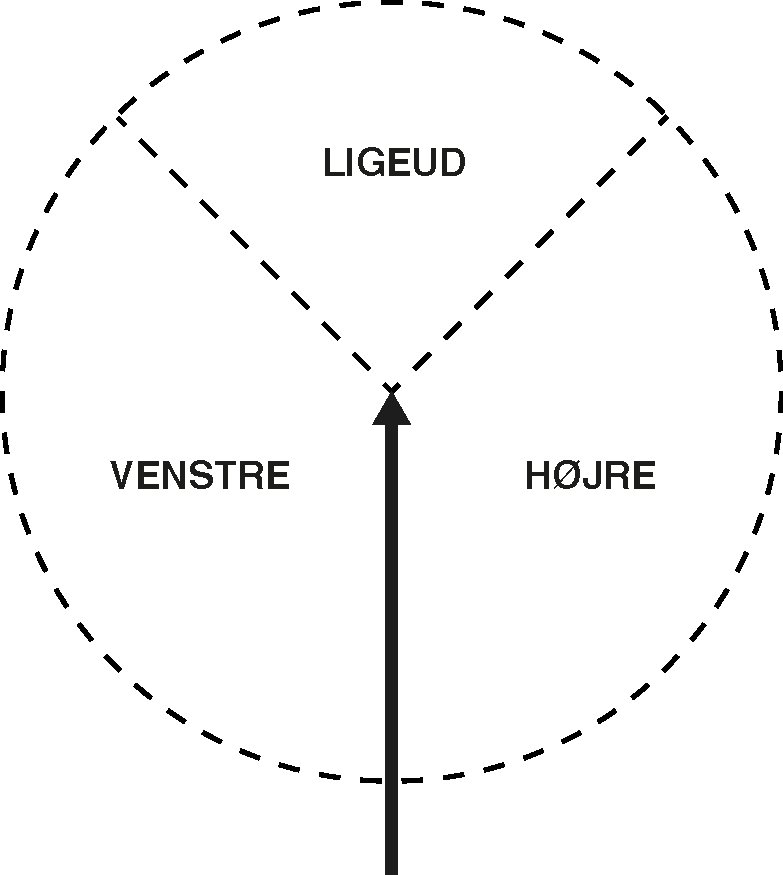
\includegraphics[width=0.4\textwidth]{tekstuelRepraesentation1}
	\captionsetup{width=0.8\textwidth}
	\caption{Definition af typer af vejskifte.}
	\label{figur:tekstuelRepraesentation1}
\end{figure}